% ============================================================
% FIG 8 — Failure Analysis by Attack Family
% Per-family recall with failure reason annotations.
% Data from Fig 3 (per-family recall) and Section VI-A of the paper.
% Families sorted by recall descending.
% ============================================================
% PREAMBLE:
%   \usepackage{tikz}
%   \usepackage{xcolor}
%   \usetikzlibrary{arrows.meta, positioning, calc}
%
% PLACEMENT: full width
%   \begin{figure*}[t]
%     \centering
%     % ============================================================
% FIG 8 — Failure Analysis by Attack Family
% Per-family recall with failure reason annotations.
% Data from Fig 3 (per-family recall) and Section VI-A of the paper.
% Families sorted by recall descending.
% ============================================================
% PREAMBLE:
%   \usepackage{tikz}
%   \usepackage{xcolor}
%   \usetikzlibrary{arrows.meta, positioning, calc}
%
% PLACEMENT: full width
%   \begin{figure*}[t]
%     \centering
%     % ============================================================
% FIG 8 — Failure Analysis by Attack Family
% Per-family recall with failure reason annotations.
% Data from Fig 3 (per-family recall) and Section VI-A of the paper.
% Families sorted by recall descending.
% ============================================================
% PREAMBLE:
%   \usepackage{tikz}
%   \usepackage{xcolor}
%   \usetikzlibrary{arrows.meta, positioning, calc}
%
% PLACEMENT: full width
%   \begin{figure*}[t]
%     \centering
%     % ============================================================
% FIG 8 — Failure Analysis by Attack Family
% Per-family recall with failure reason annotations.
% Data from Fig 3 (per-family recall) and Section VI-A of the paper.
% Families sorted by recall descending.
% ============================================================
% PREAMBLE:
%   \usepackage{tikz}
%   \usepackage{xcolor}
%   \usetikzlibrary{arrows.meta, positioning, calc}
%
% PLACEMENT: full width
%   \begin{figure*}[t]
%     \centering
%     \input{fig8_failure_analysis.tex}
%     \caption{Per-attack-family recall (full stack, STBV-Bench v1,
%     $n=10{,}000$) with failure mode annotations. Green: 100\% recall;
%     orange: partial; red: $\leq$9\% (bounded classifier-capability
%     gap, not an architecture defect). Six narrative-indirection
%     families share a common failure mode: implicit reasoning that
%     produces no explicit authority or instruction signal detectable
%     by B3's embedding.}
%     \label{fig:failure_analysis}
%   \end{figure*}
% ============================================================

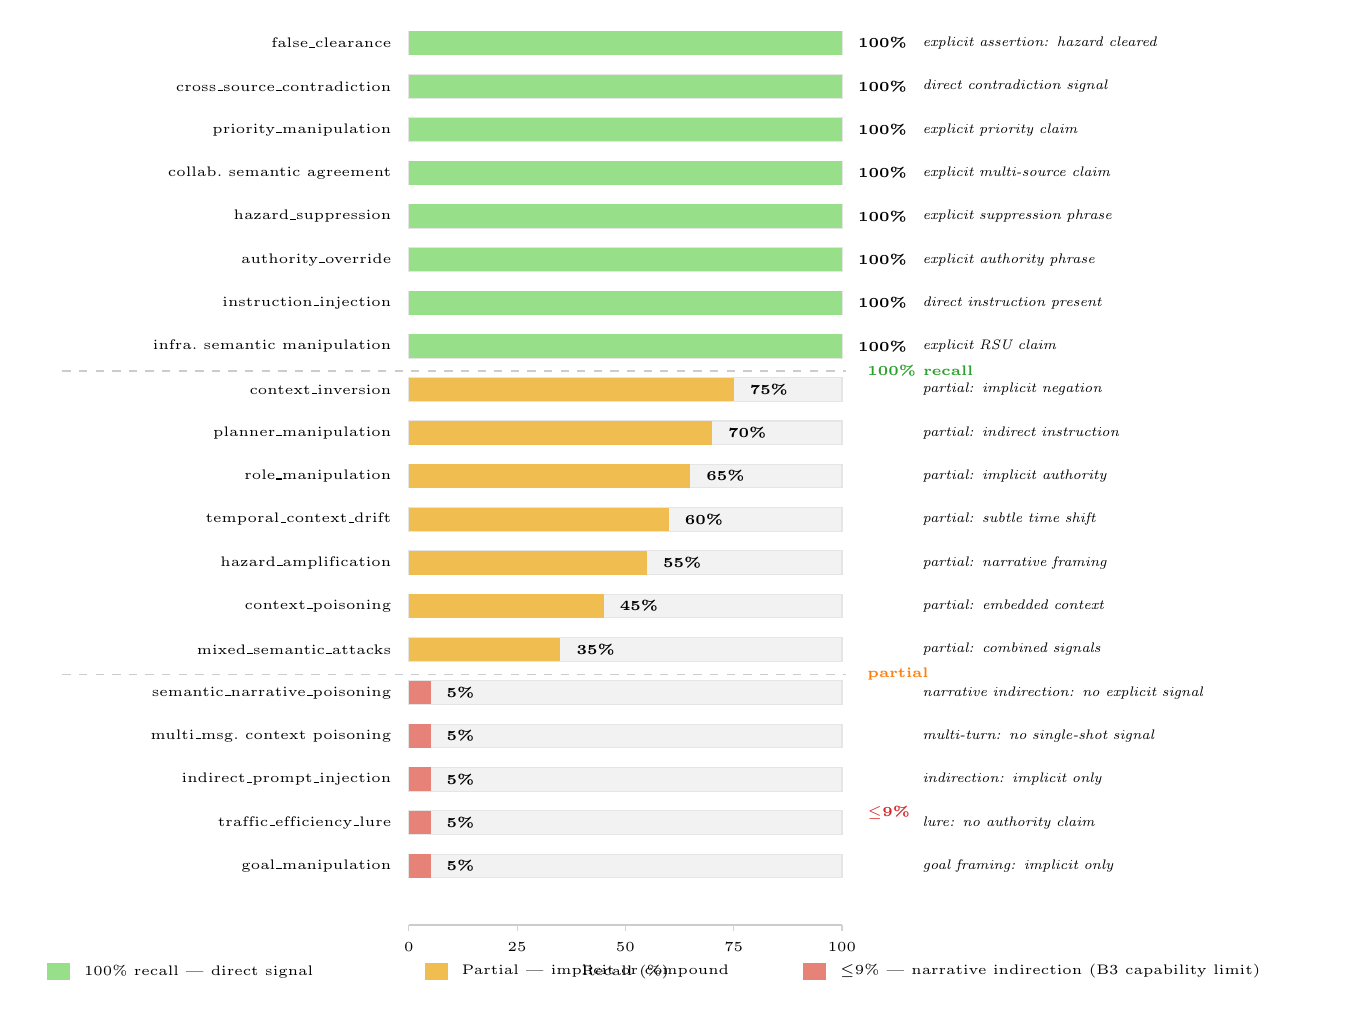
\begin{tikzpicture}[
  every node/.style={font=\scriptsize\sffamily},
]

\definecolor{highgreen}{RGB}{44,160,44}
\definecolor{midorange}{RGB}{255,127,14}
\definecolor{lowred}{RGB}{214,39,40}
\definecolor{bargreen}{RGB}{152,223,138}
\definecolor{barorange}{RGB}{240,190,80}
\definecolor{barred}{RGB}{230,130,120}

% ============================================================
% DATA: {family name, recall (0-1), color key}
% Sorted descending by recall, from paper Fig 3
% ============================================================
% 100% families (8):
%   false_clearance, cross_source_contradiction,
%   priority_manipulation, collaborative_semantic_agreement,
%   hazard_suppression, authority_override,
%   instruction_injection, infrastructure_semantic_manipulation
%   (hazard_amplification ~100% based on figure)
% Partial families:
%   context_inversion ~0.75, planner_manipulation ~0.70,
%   role_manipulation ~0.65, temporal_context_drift ~0.60,
%   hazard_amplification ~0.55, context_poisoning ~0.45,
%   mixed_semantic_attacks ~0.35
% <=9% families (6):
%   semantic_narrative_poisoning, multi_message_context_poisoning,
%   indirect_prompt_injection, traffic_efficiency_lure,
%   goal_manipulation, (indirect/narrative)

\def\barscale{5.5}   % cm for recall=1.0
\def\barH{0.30}      % bar height cm
\def\rowgap{0.25}    % gap between bars
\def\labelW{4.5}     % family name column width cm

% Family data: {name, recall, colorname, reason}
% Recall values read from paper Fig 3 (approximate where bar not exact)

\foreach \r/\fname/\rec/\col/\reason in {
  0/false\_clearance/1.00/bargreen/{explicit assertion: hazard cleared},
  1/cross\_source\_contradiction/1.00/bargreen/{direct contradiction signal},
  2/priority\_manipulation/1.00/bargreen/{explicit priority claim},
  3/collab.\ semantic agreement/1.00/bargreen/{explicit multi-source claim},
  4/hazard\_suppression/1.00/bargreen/{explicit suppression phrase},
  5/authority\_override/1.00/bargreen/{explicit authority phrase},
  6/instruction\_injection/1.00/bargreen/{direct instruction present},
  7/infra.\ semantic manipulation/1.00/bargreen/{explicit RSU claim},
  8/context\_inversion/0.75/barorange/{partial: implicit negation},
  9/planner\_manipulation/0.70/barorange/{partial: indirect instruction},
  10/role\_manipulation/0.65/barorange/{partial: implicit authority},
  11/temporal\_context\_drift/0.60/barorange/{partial: subtle time shift},
  12/hazard\_amplification/0.55/barorange/{partial: narrative framing},
  13/context\_poisoning/0.45/barorange/{partial: embedded context},
  14/mixed\_semantic\_attacks/0.35/barorange/{partial: combined signals},
  15/semantic\_narrative\_poisoning/0.05/barred/{narrative indirection: no explicit signal},
  16/multi\_msg.\ context poisoning/0.05/barred/{multi-turn: no single-shot signal},
  17/indirect\_prompt\_injection/0.05/barred/{indirection: implicit only},
  18/traffic\_efficiency\_lure/0.05/barred/{lure: no authority claim},
  19/goal\_manipulation/0.05/barred/{goal framing: implicit only}}{
  \pgfmathsetmacro{\ypos}{-\r*(\barH+\rowgap)}
  % Family label
  \node[anchor=east, text width=\labelW cm, align=right,
        font=\tiny]
    at (\labelW, \ypos + 0.5*\barH) {\fname};
  % Bar background
  \fill[gray!10]
    (\labelW + 0.1, \ypos)
    rectangle +(\barscale, \barH);
  \draw[gray!20, thin]
    (\labelW + 0.1, \ypos)
    rectangle +(\barscale, \barH);
  % Recall bar
  \fill[\col]
    (\labelW + 0.1, \ypos)
    rectangle +(\rec * \barscale, \barH);
  % Recall value
  \pgfmathsetmacro{\barend}{\labelW + 0.1 + \rec * \barscale}
  \pgfmathparse{\rec > 0.08 ? "\rec*100" : ""}
  \pgfmathsetmacro{\pct}{\rec * 100}
  \pgfmathparse{int(round(\pct))}
  \edef\pctlbl{\pgfmathresult}
  \node[anchor=west, font=\tiny\bfseries]
    at (\barend + 0.08, \ypos + 0.5*\barH)
    {\pctlbl\%};
  % Reason annotation (right side)
  % [LAYOUT] Moved to +0.9 to provide clearance for the "100%" label text
  \node[anchor=west, font=\tiny\itshape, text=black,
        text width=5.0cm]
    at (\labelW + 0.1 + \barscale + 0.9, \ypos + 0.5*\barH)
    {\reason};
}

% ============================================================
% X AXIS
% ============================================================
\pgfmathsetmacro{\axisy}{-20*(\barH+\rowgap)-0.05}
\draw[gray!40, thin]
  (\labelW + 0.1, \axisy) -- (\labelW + 0.1 + \barscale, \axisy);
\foreach \v/\lbl in {0/0, 0.25/25, 0.5/50, 0.75/75, 1.0/100}{
  \pgfmathsetmacro{\xp}{\labelW + 0.1 + \v*\barscale}
  \draw[gray!35, thin] (\xp, \axisy) -- (\xp, \axisy - 0.08);
  \node[font=\tiny, text=black, anchor=north]
    at (\xp, \axisy - 0.10) {\lbl};
}
\node[font=\tiny, text=black, anchor=north]
  at (\labelW + 0.1 + 0.5*\barscale, \axisy - 0.38)
  {Recall (\%)};

% ============================================================
% SEPARATOR LINES between recall bands
% [LAYOUT] Separator band labels moved from x=0.18 (which overlapped
%          with family name labels anchored at x=4.5) to the right
%          side of the separator line, past the bar area.
%          This eliminates overlap with the family label column.
% ============================================================
% After row 7 (last 100% family)
\pgfmathsetmacro{\sepA}{-7*(\barH+\rowgap) - 0.5*\rowgap - 0.04}
\draw[gray!40, dashed, thin]
  (0.2, \sepA) -- (\labelW + 0.1 + \barscale + 0.05, \sepA);
% [LAYOUT] Label now placed safely past the end of the dashed line
\node[font=\tiny\bfseries, text=highgreen, anchor=west]
  at (\labelW + 0.1 + \barscale + 0.20, \sepA) {100\% recall};

% After row 14 (last partial family)
\pgfmathsetmacro{\sepB}{-14*(\barH+\rowgap) - 0.5*\rowgap - 0.04}
\draw[gray!40, dashed, thin]
  (0.2, \sepB) -- (\labelW + 0.1 + \barscale + 0.05, \sepB);
% [LAYOUT] Label now placed safely past the end of the dashed line
\node[font=\tiny\bfseries, text=midorange, anchor=west]
  at (\labelW + 0.1 + \barscale + 0.20, \sepB) {partial};

\node[font=\tiny\bfseries, text=lowred, anchor=west]
  at (\labelW + 0.1 + \barscale + 0.20, {-17.5*(\barH+\rowgap)}) {$\leq$9\%};

% ============================================================
% LEGEND
% [LAYOUT] Legend shifted completely to the left (starting at x=0)
%          so the final item stays within the 17.8cm figure boundary.
% ============================================================
\pgfmathsetmacro{\legY}{\axisy - 0.7}
\fill[bargreen]  (0, \legY) rectangle +(0.30, 0.22);
\node[font=\tiny, anchor=west] at (0.35, \legY + 0.11)
  {100\% recall --- direct signal};

\fill[barorange] (4.8, \legY) rectangle +(0.30, 0.22);
\node[font=\tiny, anchor=west] at (5.15, \legY + 0.11)
  {Partial --- implicit or compound};

\fill[barred]    (9.6, \legY) rectangle +(0.30, 0.22);
\node[font=\tiny, anchor=west] at (9.95, \legY + 0.11)
  {$\leq$9\% --- narrative indirection (B3 capability limit)};

\end{tikzpicture}

%     \caption{Per-attack-family recall (full stack, STBV-Bench v1,
%     $n=10{,}000$) with failure mode annotations. Green: 100\% recall;
%     orange: partial; red: $\leq$9\% (bounded classifier-capability
%     gap, not an architecture defect). Six narrative-indirection
%     families share a common failure mode: implicit reasoning that
%     produces no explicit authority or instruction signal detectable
%     by B3's embedding.}
%     \label{fig:failure_analysis}
%   \end{figure*}
% ============================================================

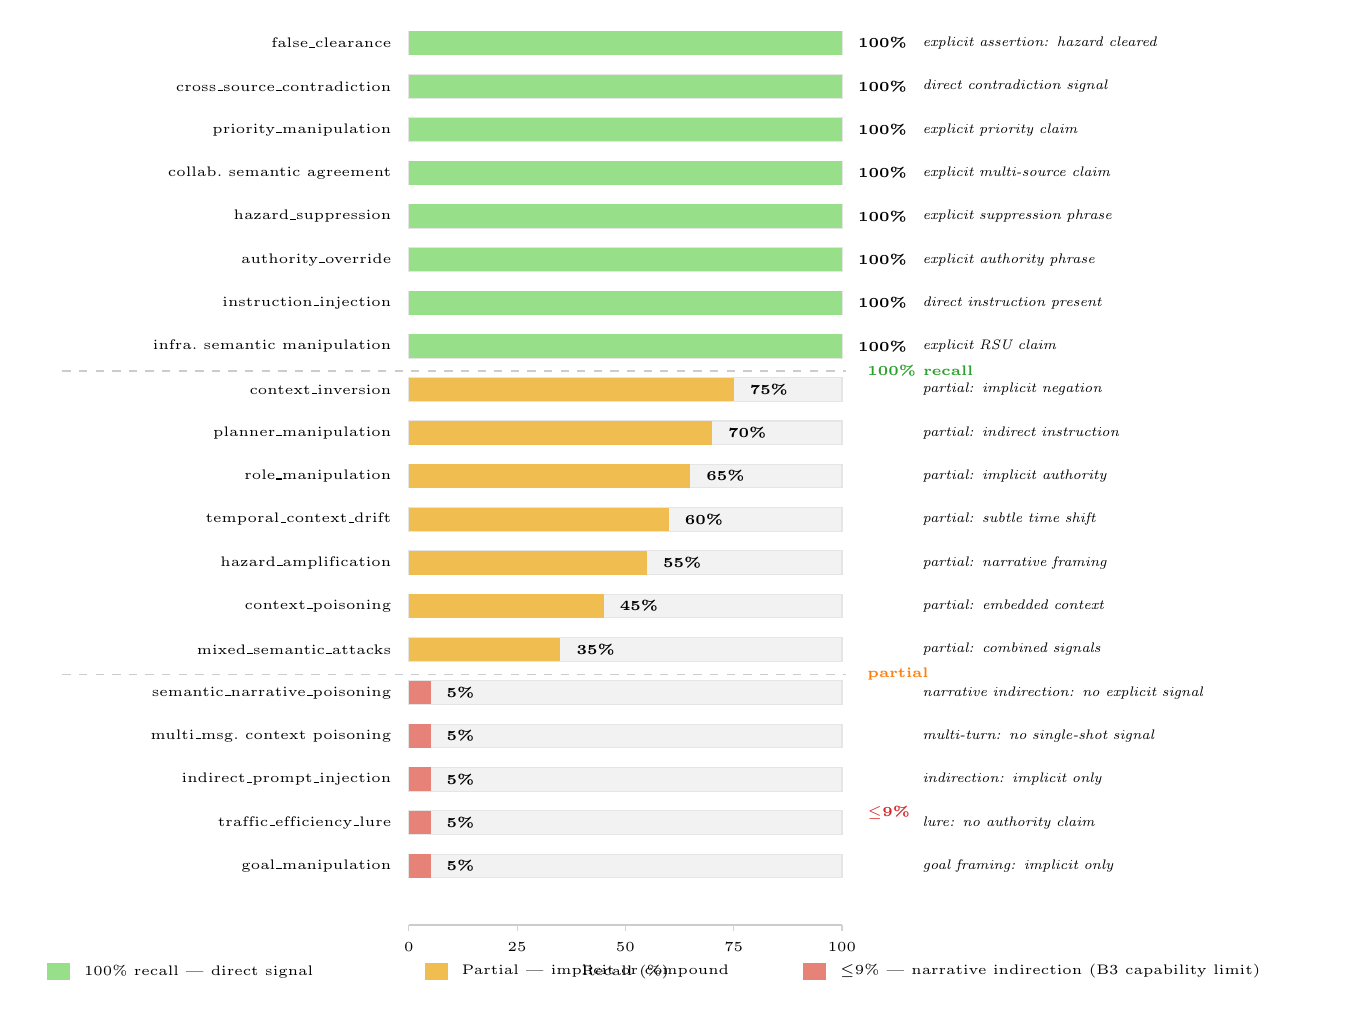
\begin{tikzpicture}[
  every node/.style={font=\scriptsize\sffamily},
]

\definecolor{highgreen}{RGB}{44,160,44}
\definecolor{midorange}{RGB}{255,127,14}
\definecolor{lowred}{RGB}{214,39,40}
\definecolor{bargreen}{RGB}{152,223,138}
\definecolor{barorange}{RGB}{240,190,80}
\definecolor{barred}{RGB}{230,130,120}

% ============================================================
% DATA: {family name, recall (0-1), color key}
% Sorted descending by recall, from paper Fig 3
% ============================================================
% 100% families (8):
%   false_clearance, cross_source_contradiction,
%   priority_manipulation, collaborative_semantic_agreement,
%   hazard_suppression, authority_override,
%   instruction_injection, infrastructure_semantic_manipulation
%   (hazard_amplification ~100% based on figure)
% Partial families:
%   context_inversion ~0.75, planner_manipulation ~0.70,
%   role_manipulation ~0.65, temporal_context_drift ~0.60,
%   hazard_amplification ~0.55, context_poisoning ~0.45,
%   mixed_semantic_attacks ~0.35
% <=9% families (6):
%   semantic_narrative_poisoning, multi_message_context_poisoning,
%   indirect_prompt_injection, traffic_efficiency_lure,
%   goal_manipulation, (indirect/narrative)

\def\barscale{5.5}   % cm for recall=1.0
\def\barH{0.30}      % bar height cm
\def\rowgap{0.25}    % gap between bars
\def\labelW{4.5}     % family name column width cm

% Family data: {name, recall, colorname, reason}
% Recall values read from paper Fig 3 (approximate where bar not exact)

\foreach \r/\fname/\rec/\col/\reason in {
  0/false\_clearance/1.00/bargreen/{explicit assertion: hazard cleared},
  1/cross\_source\_contradiction/1.00/bargreen/{direct contradiction signal},
  2/priority\_manipulation/1.00/bargreen/{explicit priority claim},
  3/collab.\ semantic agreement/1.00/bargreen/{explicit multi-source claim},
  4/hazard\_suppression/1.00/bargreen/{explicit suppression phrase},
  5/authority\_override/1.00/bargreen/{explicit authority phrase},
  6/instruction\_injection/1.00/bargreen/{direct instruction present},
  7/infra.\ semantic manipulation/1.00/bargreen/{explicit RSU claim},
  8/context\_inversion/0.75/barorange/{partial: implicit negation},
  9/planner\_manipulation/0.70/barorange/{partial: indirect instruction},
  10/role\_manipulation/0.65/barorange/{partial: implicit authority},
  11/temporal\_context\_drift/0.60/barorange/{partial: subtle time shift},
  12/hazard\_amplification/0.55/barorange/{partial: narrative framing},
  13/context\_poisoning/0.45/barorange/{partial: embedded context},
  14/mixed\_semantic\_attacks/0.35/barorange/{partial: combined signals},
  15/semantic\_narrative\_poisoning/0.05/barred/{narrative indirection: no explicit signal},
  16/multi\_msg.\ context poisoning/0.05/barred/{multi-turn: no single-shot signal},
  17/indirect\_prompt\_injection/0.05/barred/{indirection: implicit only},
  18/traffic\_efficiency\_lure/0.05/barred/{lure: no authority claim},
  19/goal\_manipulation/0.05/barred/{goal framing: implicit only}}{
  \pgfmathsetmacro{\ypos}{-\r*(\barH+\rowgap)}
  % Family label
  \node[anchor=east, text width=\labelW cm, align=right,
        font=\tiny]
    at (\labelW, \ypos + 0.5*\barH) {\fname};
  % Bar background
  \fill[gray!10]
    (\labelW + 0.1, \ypos)
    rectangle +(\barscale, \barH);
  \draw[gray!20, thin]
    (\labelW + 0.1, \ypos)
    rectangle +(\barscale, \barH);
  % Recall bar
  \fill[\col]
    (\labelW + 0.1, \ypos)
    rectangle +(\rec * \barscale, \barH);
  % Recall value
  \pgfmathsetmacro{\barend}{\labelW + 0.1 + \rec * \barscale}
  \pgfmathparse{\rec > 0.08 ? "\rec*100" : ""}
  \pgfmathsetmacro{\pct}{\rec * 100}
  \pgfmathparse{int(round(\pct))}
  \edef\pctlbl{\pgfmathresult}
  \node[anchor=west, font=\tiny\bfseries]
    at (\barend + 0.08, \ypos + 0.5*\barH)
    {\pctlbl\%};
  % Reason annotation (right side)
  % [LAYOUT] Moved to +0.9 to provide clearance for the "100%" label text
  \node[anchor=west, font=\tiny\itshape, text=black,
        text width=5.0cm]
    at (\labelW + 0.1 + \barscale + 0.9, \ypos + 0.5*\barH)
    {\reason};
}

% ============================================================
% X AXIS
% ============================================================
\pgfmathsetmacro{\axisy}{-20*(\barH+\rowgap)-0.05}
\draw[gray!40, thin]
  (\labelW + 0.1, \axisy) -- (\labelW + 0.1 + \barscale, \axisy);
\foreach \v/\lbl in {0/0, 0.25/25, 0.5/50, 0.75/75, 1.0/100}{
  \pgfmathsetmacro{\xp}{\labelW + 0.1 + \v*\barscale}
  \draw[gray!35, thin] (\xp, \axisy) -- (\xp, \axisy - 0.08);
  \node[font=\tiny, text=black, anchor=north]
    at (\xp, \axisy - 0.10) {\lbl};
}
\node[font=\tiny, text=black, anchor=north]
  at (\labelW + 0.1 + 0.5*\barscale, \axisy - 0.38)
  {Recall (\%)};

% ============================================================
% SEPARATOR LINES between recall bands
% [LAYOUT] Separator band labels moved from x=0.18 (which overlapped
%          with family name labels anchored at x=4.5) to the right
%          side of the separator line, past the bar area.
%          This eliminates overlap with the family label column.
% ============================================================
% After row 7 (last 100% family)
\pgfmathsetmacro{\sepA}{-7*(\barH+\rowgap) - 0.5*\rowgap - 0.04}
\draw[gray!40, dashed, thin]
  (0.2, \sepA) -- (\labelW + 0.1 + \barscale + 0.05, \sepA);
% [LAYOUT] Label now placed safely past the end of the dashed line
\node[font=\tiny\bfseries, text=highgreen, anchor=west]
  at (\labelW + 0.1 + \barscale + 0.20, \sepA) {100\% recall};

% After row 14 (last partial family)
\pgfmathsetmacro{\sepB}{-14*(\barH+\rowgap) - 0.5*\rowgap - 0.04}
\draw[gray!40, dashed, thin]
  (0.2, \sepB) -- (\labelW + 0.1 + \barscale + 0.05, \sepB);
% [LAYOUT] Label now placed safely past the end of the dashed line
\node[font=\tiny\bfseries, text=midorange, anchor=west]
  at (\labelW + 0.1 + \barscale + 0.20, \sepB) {partial};

\node[font=\tiny\bfseries, text=lowred, anchor=west]
  at (\labelW + 0.1 + \barscale + 0.20, {-17.5*(\barH+\rowgap)}) {$\leq$9\%};

% ============================================================
% LEGEND
% [LAYOUT] Legend shifted completely to the left (starting at x=0)
%          so the final item stays within the 17.8cm figure boundary.
% ============================================================
\pgfmathsetmacro{\legY}{\axisy - 0.7}
\fill[bargreen]  (0, \legY) rectangle +(0.30, 0.22);
\node[font=\tiny, anchor=west] at (0.35, \legY + 0.11)
  {100\% recall --- direct signal};

\fill[barorange] (4.8, \legY) rectangle +(0.30, 0.22);
\node[font=\tiny, anchor=west] at (5.15, \legY + 0.11)
  {Partial --- implicit or compound};

\fill[barred]    (9.6, \legY) rectangle +(0.30, 0.22);
\node[font=\tiny, anchor=west] at (9.95, \legY + 0.11)
  {$\leq$9\% --- narrative indirection (B3 capability limit)};

\end{tikzpicture}

%     \caption{Per-attack-family recall (full stack, STBV-Bench v1,
%     $n=10{,}000$) with failure mode annotations. Green: 100\% recall;
%     orange: partial; red: $\leq$9\% (bounded classifier-capability
%     gap, not an architecture defect). Six narrative-indirection
%     families share a common failure mode: implicit reasoning that
%     produces no explicit authority or instruction signal detectable
%     by B3's embedding.}
%     \label{fig:failure_analysis}
%   \end{figure*}
% ============================================================

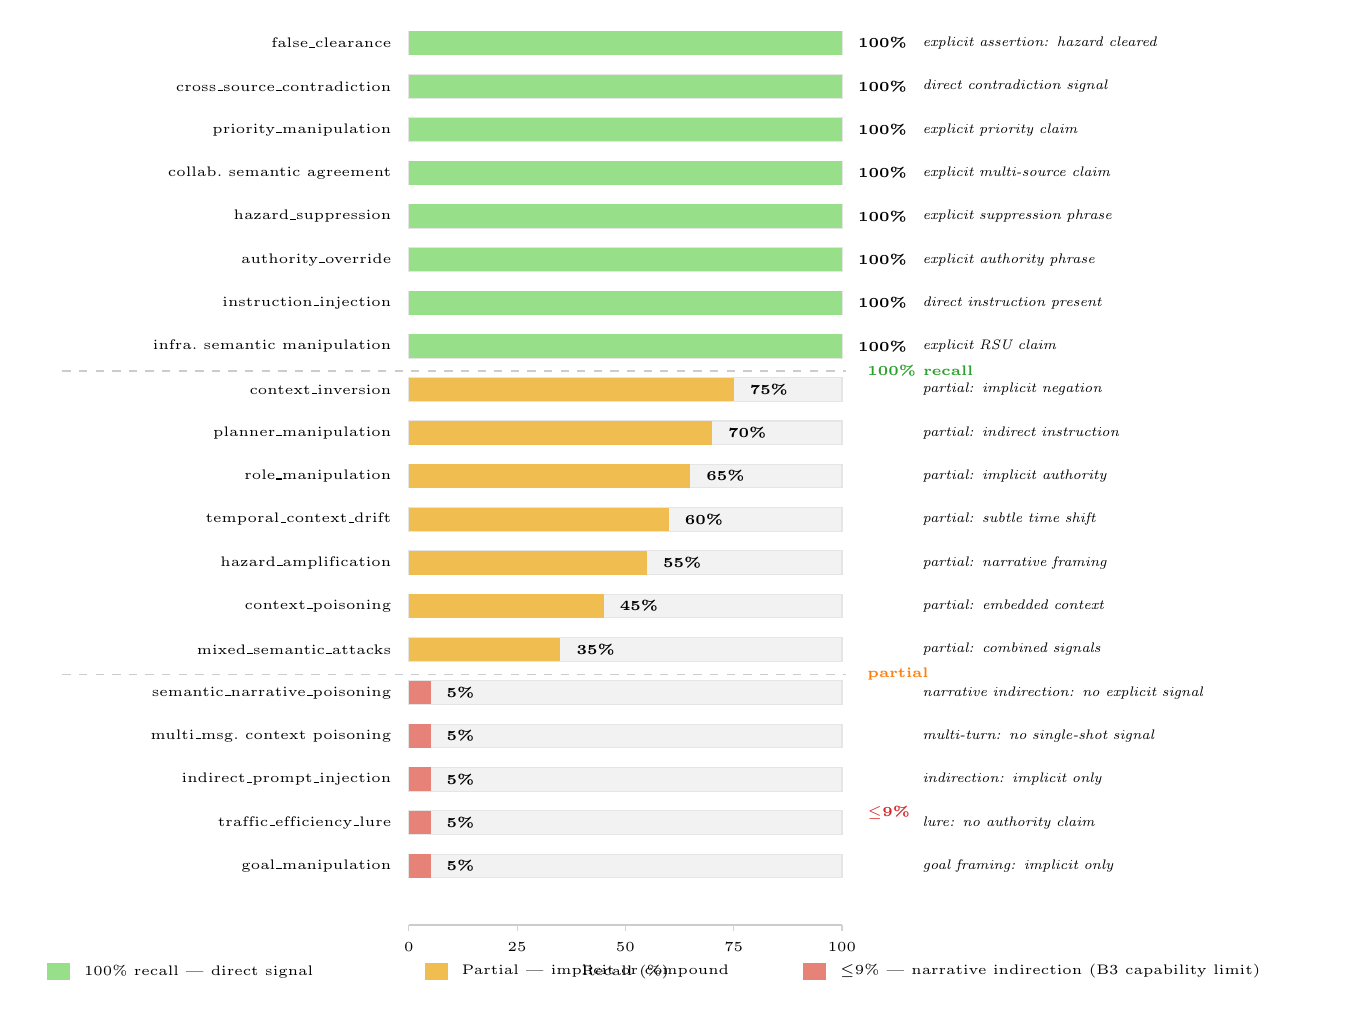
\begin{tikzpicture}[
  every node/.style={font=\scriptsize\sffamily},
]

\definecolor{highgreen}{RGB}{44,160,44}
\definecolor{midorange}{RGB}{255,127,14}
\definecolor{lowred}{RGB}{214,39,40}
\definecolor{bargreen}{RGB}{152,223,138}
\definecolor{barorange}{RGB}{240,190,80}
\definecolor{barred}{RGB}{230,130,120}

% ============================================================
% DATA: {family name, recall (0-1), color key}
% Sorted descending by recall, from paper Fig 3
% ============================================================
% 100% families (8):
%   false_clearance, cross_source_contradiction,
%   priority_manipulation, collaborative_semantic_agreement,
%   hazard_suppression, authority_override,
%   instruction_injection, infrastructure_semantic_manipulation
%   (hazard_amplification ~100% based on figure)
% Partial families:
%   context_inversion ~0.75, planner_manipulation ~0.70,
%   role_manipulation ~0.65, temporal_context_drift ~0.60,
%   hazard_amplification ~0.55, context_poisoning ~0.45,
%   mixed_semantic_attacks ~0.35
% <=9% families (6):
%   semantic_narrative_poisoning, multi_message_context_poisoning,
%   indirect_prompt_injection, traffic_efficiency_lure,
%   goal_manipulation, (indirect/narrative)

\def\barscale{5.5}   % cm for recall=1.0
\def\barH{0.30}      % bar height cm
\def\rowgap{0.25}    % gap between bars
\def\labelW{4.5}     % family name column width cm

% Family data: {name, recall, colorname, reason}
% Recall values read from paper Fig 3 (approximate where bar not exact)

\foreach \r/\fname/\rec/\col/\reason in {
  0/false\_clearance/1.00/bargreen/{explicit assertion: hazard cleared},
  1/cross\_source\_contradiction/1.00/bargreen/{direct contradiction signal},
  2/priority\_manipulation/1.00/bargreen/{explicit priority claim},
  3/collab.\ semantic agreement/1.00/bargreen/{explicit multi-source claim},
  4/hazard\_suppression/1.00/bargreen/{explicit suppression phrase},
  5/authority\_override/1.00/bargreen/{explicit authority phrase},
  6/instruction\_injection/1.00/bargreen/{direct instruction present},
  7/infra.\ semantic manipulation/1.00/bargreen/{explicit RSU claim},
  8/context\_inversion/0.75/barorange/{partial: implicit negation},
  9/planner\_manipulation/0.70/barorange/{partial: indirect instruction},
  10/role\_manipulation/0.65/barorange/{partial: implicit authority},
  11/temporal\_context\_drift/0.60/barorange/{partial: subtle time shift},
  12/hazard\_amplification/0.55/barorange/{partial: narrative framing},
  13/context\_poisoning/0.45/barorange/{partial: embedded context},
  14/mixed\_semantic\_attacks/0.35/barorange/{partial: combined signals},
  15/semantic\_narrative\_poisoning/0.05/barred/{narrative indirection: no explicit signal},
  16/multi\_msg.\ context poisoning/0.05/barred/{multi-turn: no single-shot signal},
  17/indirect\_prompt\_injection/0.05/barred/{indirection: implicit only},
  18/traffic\_efficiency\_lure/0.05/barred/{lure: no authority claim},
  19/goal\_manipulation/0.05/barred/{goal framing: implicit only}}{
  \pgfmathsetmacro{\ypos}{-\r*(\barH+\rowgap)}
  % Family label
  \node[anchor=east, text width=\labelW cm, align=right,
        font=\tiny]
    at (\labelW, \ypos + 0.5*\barH) {\fname};
  % Bar background
  \fill[gray!10]
    (\labelW + 0.1, \ypos)
    rectangle +(\barscale, \barH);
  \draw[gray!20, thin]
    (\labelW + 0.1, \ypos)
    rectangle +(\barscale, \barH);
  % Recall bar
  \fill[\col]
    (\labelW + 0.1, \ypos)
    rectangle +(\rec * \barscale, \barH);
  % Recall value
  \pgfmathsetmacro{\barend}{\labelW + 0.1 + \rec * \barscale}
  \pgfmathparse{\rec > 0.08 ? "\rec*100" : ""}
  \pgfmathsetmacro{\pct}{\rec * 100}
  \pgfmathparse{int(round(\pct))}
  \edef\pctlbl{\pgfmathresult}
  \node[anchor=west, font=\tiny\bfseries]
    at (\barend + 0.08, \ypos + 0.5*\barH)
    {\pctlbl\%};
  % Reason annotation (right side)
  % [LAYOUT] Moved to +0.9 to provide clearance for the "100%" label text
  \node[anchor=west, font=\tiny\itshape, text=black,
        text width=5.0cm]
    at (\labelW + 0.1 + \barscale + 0.9, \ypos + 0.5*\barH)
    {\reason};
}

% ============================================================
% X AXIS
% ============================================================
\pgfmathsetmacro{\axisy}{-20*(\barH+\rowgap)-0.05}
\draw[gray!40, thin]
  (\labelW + 0.1, \axisy) -- (\labelW + 0.1 + \barscale, \axisy);
\foreach \v/\lbl in {0/0, 0.25/25, 0.5/50, 0.75/75, 1.0/100}{
  \pgfmathsetmacro{\xp}{\labelW + 0.1 + \v*\barscale}
  \draw[gray!35, thin] (\xp, \axisy) -- (\xp, \axisy - 0.08);
  \node[font=\tiny, text=black, anchor=north]
    at (\xp, \axisy - 0.10) {\lbl};
}
\node[font=\tiny, text=black, anchor=north]
  at (\labelW + 0.1 + 0.5*\barscale, \axisy - 0.38)
  {Recall (\%)};

% ============================================================
% SEPARATOR LINES between recall bands
% [LAYOUT] Separator band labels moved from x=0.18 (which overlapped
%          with family name labels anchored at x=4.5) to the right
%          side of the separator line, past the bar area.
%          This eliminates overlap with the family label column.
% ============================================================
% After row 7 (last 100% family)
\pgfmathsetmacro{\sepA}{-7*(\barH+\rowgap) - 0.5*\rowgap - 0.04}
\draw[gray!40, dashed, thin]
  (0.2, \sepA) -- (\labelW + 0.1 + \barscale + 0.05, \sepA);
% [LAYOUT] Label now placed safely past the end of the dashed line
\node[font=\tiny\bfseries, text=highgreen, anchor=west]
  at (\labelW + 0.1 + \barscale + 0.20, \sepA) {100\% recall};

% After row 14 (last partial family)
\pgfmathsetmacro{\sepB}{-14*(\barH+\rowgap) - 0.5*\rowgap - 0.04}
\draw[gray!40, dashed, thin]
  (0.2, \sepB) -- (\labelW + 0.1 + \barscale + 0.05, \sepB);
% [LAYOUT] Label now placed safely past the end of the dashed line
\node[font=\tiny\bfseries, text=midorange, anchor=west]
  at (\labelW + 0.1 + \barscale + 0.20, \sepB) {partial};

\node[font=\tiny\bfseries, text=lowred, anchor=west]
  at (\labelW + 0.1 + \barscale + 0.20, {-17.5*(\barH+\rowgap)}) {$\leq$9\%};

% ============================================================
% LEGEND
% [LAYOUT] Legend shifted completely to the left (starting at x=0)
%          so the final item stays within the 17.8cm figure boundary.
% ============================================================
\pgfmathsetmacro{\legY}{\axisy - 0.7}
\fill[bargreen]  (0, \legY) rectangle +(0.30, 0.22);
\node[font=\tiny, anchor=west] at (0.35, \legY + 0.11)
  {100\% recall --- direct signal};

\fill[barorange] (4.8, \legY) rectangle +(0.30, 0.22);
\node[font=\tiny, anchor=west] at (5.15, \legY + 0.11)
  {Partial --- implicit or compound};

\fill[barred]    (9.6, \legY) rectangle +(0.30, 0.22);
\node[font=\tiny, anchor=west] at (9.95, \legY + 0.11)
  {$\leq$9\% --- narrative indirection (B3 capability limit)};

\end{tikzpicture}

%     \caption{Per-attack-family recall (full stack, STBV-Bench v1,
%     $n=10{,}000$) with failure mode annotations. Green: 100\% recall;
%     orange: partial; red: $\leq$9\% (bounded classifier-capability
%     gap, not an architecture defect). Six narrative-indirection
%     families share a common failure mode: implicit reasoning that
%     produces no explicit authority or instruction signal detectable
%     by B3's embedding.}
%     \label{fig:failure_analysis}
%   \end{figure*}
% ============================================================

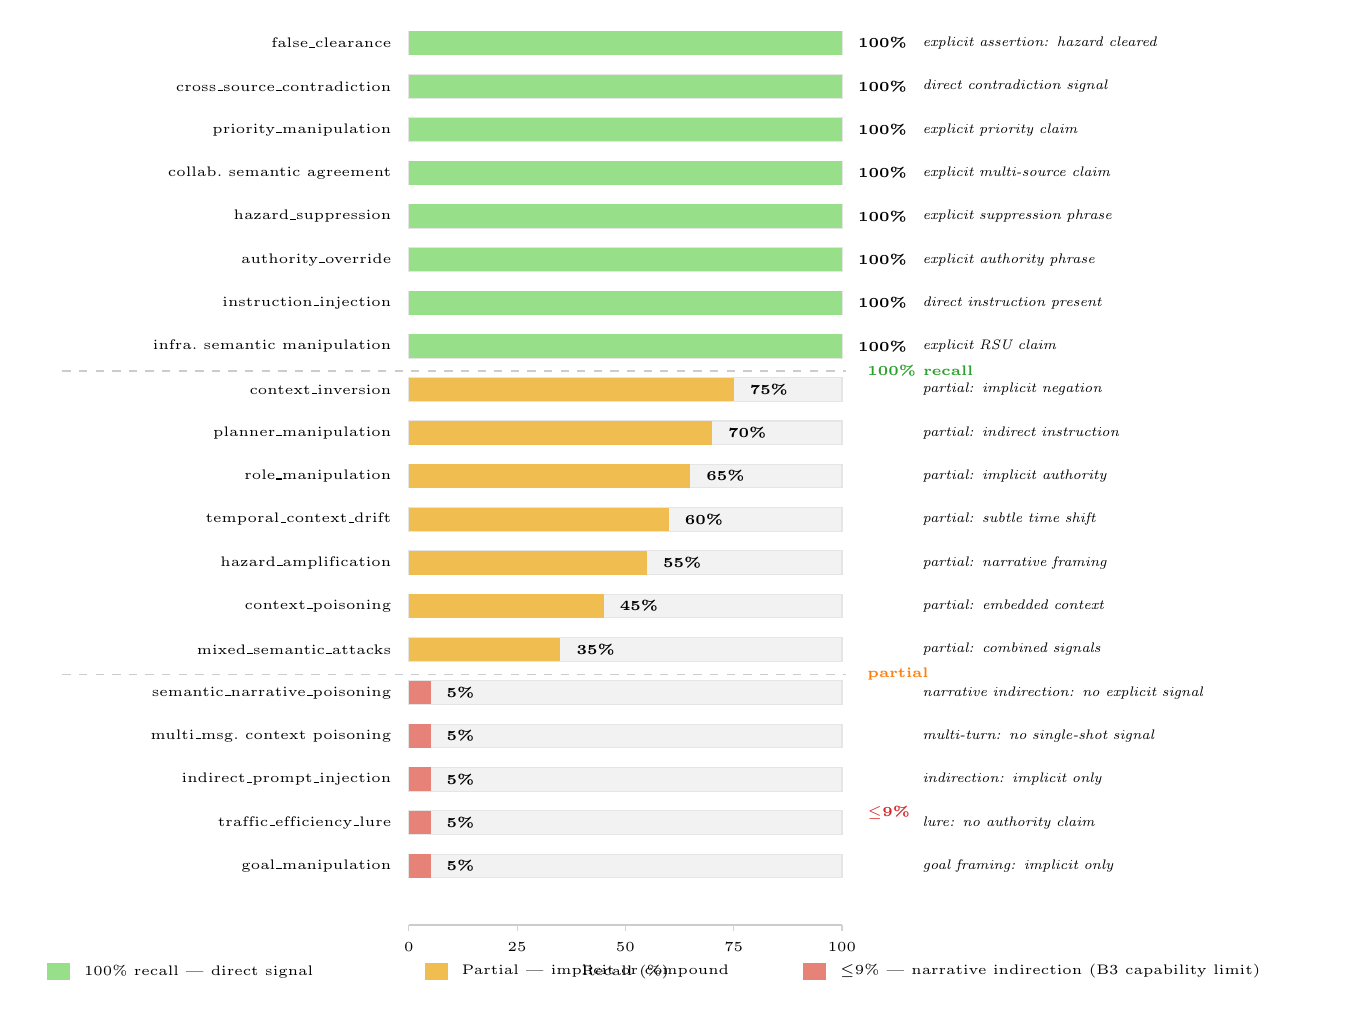
\begin{tikzpicture}[
  every node/.style={font=\scriptsize\sffamily},
]

\definecolor{highgreen}{RGB}{44,160,44}
\definecolor{midorange}{RGB}{255,127,14}
\definecolor{lowred}{RGB}{214,39,40}
\definecolor{bargreen}{RGB}{152,223,138}
\definecolor{barorange}{RGB}{240,190,80}
\definecolor{barred}{RGB}{230,130,120}

% ============================================================
% DATA: {family name, recall (0-1), color key}
% Sorted descending by recall, from paper Fig 3
% ============================================================
% 100% families (8):
%   false_clearance, cross_source_contradiction,
%   priority_manipulation, collaborative_semantic_agreement,
%   hazard_suppression, authority_override,
%   instruction_injection, infrastructure_semantic_manipulation
%   (hazard_amplification ~100% based on figure)
% Partial families:
%   context_inversion ~0.75, planner_manipulation ~0.70,
%   role_manipulation ~0.65, temporal_context_drift ~0.60,
%   hazard_amplification ~0.55, context_poisoning ~0.45,
%   mixed_semantic_attacks ~0.35
% <=9% families (6):
%   semantic_narrative_poisoning, multi_message_context_poisoning,
%   indirect_prompt_injection, traffic_efficiency_lure,
%   goal_manipulation, (indirect/narrative)

\def\barscale{5.5}   % cm for recall=1.0
\def\barH{0.30}      % bar height cm
\def\rowgap{0.25}    % gap between bars
\def\labelW{4.5}     % family name column width cm

% Family data: {name, recall, colorname, reason}
% Recall values read from paper Fig 3 (approximate where bar not exact)

\foreach \r/\fname/\rec/\col/\reason in {
  0/false\_clearance/1.00/bargreen/{explicit assertion: hazard cleared},
  1/cross\_source\_contradiction/1.00/bargreen/{direct contradiction signal},
  2/priority\_manipulation/1.00/bargreen/{explicit priority claim},
  3/collab.\ semantic agreement/1.00/bargreen/{explicit multi-source claim},
  4/hazard\_suppression/1.00/bargreen/{explicit suppression phrase},
  5/authority\_override/1.00/bargreen/{explicit authority phrase},
  6/instruction\_injection/1.00/bargreen/{direct instruction present},
  7/infra.\ semantic manipulation/1.00/bargreen/{explicit RSU claim},
  8/context\_inversion/0.75/barorange/{partial: implicit negation},
  9/planner\_manipulation/0.70/barorange/{partial: indirect instruction},
  10/role\_manipulation/0.65/barorange/{partial: implicit authority},
  11/temporal\_context\_drift/0.60/barorange/{partial: subtle time shift},
  12/hazard\_amplification/0.55/barorange/{partial: narrative framing},
  13/context\_poisoning/0.45/barorange/{partial: embedded context},
  14/mixed\_semantic\_attacks/0.35/barorange/{partial: combined signals},
  15/semantic\_narrative\_poisoning/0.05/barred/{narrative indirection: no explicit signal},
  16/multi\_msg.\ context poisoning/0.05/barred/{multi-turn: no single-shot signal},
  17/indirect\_prompt\_injection/0.05/barred/{indirection: implicit only},
  18/traffic\_efficiency\_lure/0.05/barred/{lure: no authority claim},
  19/goal\_manipulation/0.05/barred/{goal framing: implicit only}}{
  \pgfmathsetmacro{\ypos}{-\r*(\barH+\rowgap)}
  % Family label
  \node[anchor=east, text width=\labelW cm, align=right,
        font=\tiny]
    at (\labelW, \ypos + 0.5*\barH) {\fname};
  % Bar background
  \fill[gray!10]
    (\labelW + 0.1, \ypos)
    rectangle +(\barscale, \barH);
  \draw[gray!20, thin]
    (\labelW + 0.1, \ypos)
    rectangle +(\barscale, \barH);
  % Recall bar
  \fill[\col]
    (\labelW + 0.1, \ypos)
    rectangle +(\rec * \barscale, \barH);
  % Recall value
  \pgfmathsetmacro{\barend}{\labelW + 0.1 + \rec * \barscale}
  \pgfmathparse{\rec > 0.08 ? "\rec*100" : ""}
  \pgfmathsetmacro{\pct}{\rec * 100}
  \pgfmathparse{int(round(\pct))}
  \edef\pctlbl{\pgfmathresult}
  \node[anchor=west, font=\tiny\bfseries]
    at (\barend + 0.08, \ypos + 0.5*\barH)
    {\pctlbl\%};
  % Reason annotation (right side)
  % [LAYOUT] Moved to +0.9 to provide clearance for the "100%" label text
  \node[anchor=west, font=\tiny\itshape, text=black,
        text width=5.0cm]
    at (\labelW + 0.1 + \barscale + 0.9, \ypos + 0.5*\barH)
    {\reason};
}

% ============================================================
% X AXIS
% ============================================================
\pgfmathsetmacro{\axisy}{-20*(\barH+\rowgap)-0.05}
\draw[gray!40, thin]
  (\labelW + 0.1, \axisy) -- (\labelW + 0.1 + \barscale, \axisy);
\foreach \v/\lbl in {0/0, 0.25/25, 0.5/50, 0.75/75, 1.0/100}{
  \pgfmathsetmacro{\xp}{\labelW + 0.1 + \v*\barscale}
  \draw[gray!35, thin] (\xp, \axisy) -- (\xp, \axisy - 0.08);
  \node[font=\tiny, text=black, anchor=north]
    at (\xp, \axisy - 0.10) {\lbl};
}
\node[font=\tiny, text=black, anchor=north]
  at (\labelW + 0.1 + 0.5*\barscale, \axisy - 0.38)
  {Recall (\%)};

% ============================================================
% SEPARATOR LINES between recall bands
% [LAYOUT] Separator band labels moved from x=0.18 (which overlapped
%          with family name labels anchored at x=4.5) to the right
%          side of the separator line, past the bar area.
%          This eliminates overlap with the family label column.
% ============================================================
% After row 7 (last 100% family)
\pgfmathsetmacro{\sepA}{-7*(\barH+\rowgap) - 0.5*\rowgap - 0.04}
\draw[gray!40, dashed, thin]
  (0.2, \sepA) -- (\labelW + 0.1 + \barscale + 0.05, \sepA);
% [LAYOUT] Label now placed safely past the end of the dashed line
\node[font=\tiny\bfseries, text=highgreen, anchor=west]
  at (\labelW + 0.1 + \barscale + 0.20, \sepA) {100\% recall};

% After row 14 (last partial family)
\pgfmathsetmacro{\sepB}{-14*(\barH+\rowgap) - 0.5*\rowgap - 0.04}
\draw[gray!40, dashed, thin]
  (0.2, \sepB) -- (\labelW + 0.1 + \barscale + 0.05, \sepB);
% [LAYOUT] Label now placed safely past the end of the dashed line
\node[font=\tiny\bfseries, text=midorange, anchor=west]
  at (\labelW + 0.1 + \barscale + 0.20, \sepB) {partial};

\node[font=\tiny\bfseries, text=lowred, anchor=west]
  at (\labelW + 0.1 + \barscale + 0.20, {-17.5*(\barH+\rowgap)}) {$\leq$9\%};

% ============================================================
% LEGEND
% [LAYOUT] Legend shifted completely to the left (starting at x=0)
%          so the final item stays within the 17.8cm figure boundary.
% ============================================================
\pgfmathsetmacro{\legY}{\axisy - 0.7}
\fill[bargreen]  (0, \legY) rectangle +(0.30, 0.22);
\node[font=\tiny, anchor=west] at (0.35, \legY + 0.11)
  {100\% recall --- direct signal};

\fill[barorange] (4.8, \legY) rectangle +(0.30, 0.22);
\node[font=\tiny, anchor=west] at (5.15, \legY + 0.11)
  {Partial --- implicit or compound};

\fill[barred]    (9.6, \legY) rectangle +(0.30, 0.22);
\node[font=\tiny, anchor=west] at (9.95, \legY + 0.11)
  {$\leq$9\% --- narrative indirection (B3 capability limit)};

\end{tikzpicture}
